\providecommand{\main}{..}
\documentclass[../mthe-493-final-project.tex]{subfiles}

% Overall implementation of our design solution.
\begin{document}
    \chapter{Implementation}
    \label{ch:implementation}

    
    \section{Distributed Computing}
    \label{sec:distributed-computing-implementation}

    % "Performs an economic analysis on multiple solutions and uses quantitative justification when choosing solution"
    \subsection{Tool Selection}
    
    While the optimization portion of the design was being implemented, the team decided to move forward with implementing the distributed computing portion of the design solution using Axon. The decision came down to two main reasons: ease in implementing the cost structure and the lower overall economical cost.

    As mentioned in~\autoref{subsec-ete-evaluation-of-tools}, DCP's cost structure between clients and workers has the downside of having clients paying a set amount decided at the beginning of work distribution. If it were to be used in the implementation of the design solution, we would need to spend additional time and resources working with Kings Distributed Systems to create a non-trivial workaround. On the other hand, Axon's lack of a cost structure means that the team would also need to spend time implementing the cost structure form scratch. Working with Duncan would save time on implementing a cost structure, and meeting the problem description's requirements would be simpler than trying to build on top of an already complex cost structure on DCP. Thus, Axon became the clear choice in terms of lower time cost and lower complexity without trading off accuracy for the purposes of the design solution.

    Another aspect of DCP that comes from it being more of a commercial product rather than a pure research tool is the cost of using the tool in practice. According to their website and when one attempts to buy credits to deploy work on DCP, It costs around \$100 to access approximately a years worth of virtual CPU computational time~\cite{kings-ds-marketing}. On the other hand, implementing the design solution in practice using Axon doesn't have a similar cost~\cite{Mays_Axon}. Based on that, Axon also becomes the preferred choice in terms of economic cost.
    
    \subsection{Network Architecture}
    \label{ssec:network-architecture}
    % Description of approach and final code-base architecture. Our physical model. Great place for an architecture diagram.
    % Naive translation form math model to actual implementation.
    % e.g., workers are represented as machines on a network

    With the distributed computing framework chosen, the team then designed how the cost structure, optimization algorithm, and parallel learning components were going to fit into network connecting the orchestrator to the learners.

    A disclaimer regarding terminology: both the distributed computing frameworks, DCP and Axon, use the term \textit{worker} to represent a \textit{learner}~\cite{Mays_Axon}\cite{noauthor_worker_nodate}. Axon uses the term \textit{client} to represent an \textit{orchestrator}~\cite{Mays_Axon}. As such, the rest of the section will use the former terms mentioned to refer to the network nodes.

    The first task to implement the network was ensuring that the client can communicate with the workers. In Axon, the intended method of doing that programmatically is through a ``noticeboard''. It works by having workers that start up sign in to the notice board to be discovered. Then when a client connects to the noticeboard to discover them, it responds with the workers that have signed in~\cite{Mays_Axon}.

    An overview of the network nodes and their relationships can be observed in~\autoref{fig:network-flowchart}.
    
    \begin{figure}
        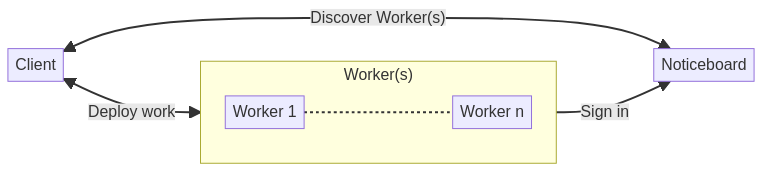
\includegraphics{network-1.png}
        \caption{Flowchart diagram of the network's architecture~\cite{group_a2_Optimization_Of_Data}.}
        \label{fig:network-flowchart}
    \end{figure}

    As far as what computers the entity's were located on, the discussion on raspberry pis versus personal computers in~\autoref{subsec-ete-evaluation-of-tools} contributed to the experimental set up involving running the nodes on personal computers for their hardware's capability to run the parallel learning tasks. Running node on a computer equates to starting python scripts as programs that can send and receive messages over their computer's local network. For simplicity, the client and noticeboard programs were ran on the same computer since the noticeboard was not computationally demanding for the small network sizes being used during experimentation.

    With the overall architecture of the network finalized, the team then implemented each of the sub components of the design solution pertaining to important steps that occur during an experiment, which can be observed in~\autoref{fig:network-sequence}.

    \begin{figure}
        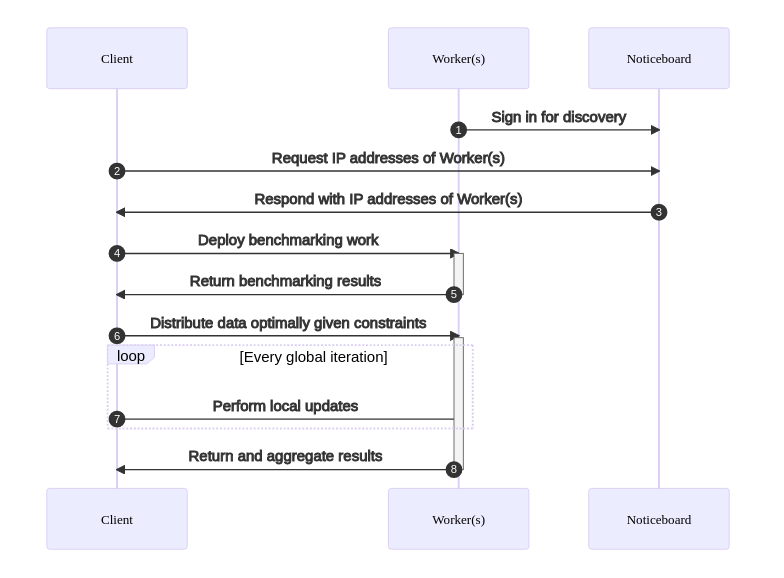
\includegraphics{network-2.png}
        \caption{Sequence diagram of an experiment~\cite{group_a2_Optimization_Of_Data}.}
        \label{fig:network-sequence}
    \end{figure}

    Steps 1 and 2 from the figure describe how the client connects to the workers mentioned earlier more precisely. The rest of the steps will form the basis of what will be discussed next in the implementation.

    But an aspect of the system that isn't shown in the sequence diagram is the cost structure. After the client discovers the workers, the teams implemented the feature by designing the client to have the ability to set each worker's recruitment cost. In a more realistic set up, each worker would set their recruitment costs, with some thought given to each of their computational capabilities. This design decision came from a need to make setting up test cases for experiments easier. Instead of spending time setting up a system to update the recruitment cost of each worker on the network outside of the client, it would be simpler to send each worker their recruitment cost from the client once they are connected~\cite{group_a2_Optimization_Of_Data}. 
        
    \subsection{Benchmarking}
    \label{ssec:benchmarking}

    The next step after the client and workers have connected and set the recruitment costs is to have the client determine the computational capabilities of each worker, i.e., steps 4 and 5 from~\autoref{fig:network-sequence}. To do so, the client sends each worker work that calculates their computational capabilities, work that Duncan has provided to the team~\cite{Mays_Benchmarking}.

    As specified by Duncan's work, each learner $l_i$ will be benchmarked to estimate an \textit{upload/download rate}, $b_i$, and a \textit{sample compute rate}, $C_i$. Each learner also has a \textit{fee} to compute a sample, $c_i$. Together, we can define the following quantities:

    \begin{itemize}
        \item \textit{Subjob download time}, $t^d_i$, which is a function of $s_i$
              \[t^d_i = \frac{P_m + P_d s_i}{b_i}\]
        \item \textit{Subjob compute time}, $t^c_i$, which is a function of $s_i$
              \[t^c_i = \frac{\tau s_i}{C_i}\]
        \item \textit{Subjob upload time}, $t^u_i$, which is fixed for a given job
              \[t^u_i = \frac{P_m}{b_i}\]
    \end{itemize}

    A learner's \textit{global cycle time} to compute a subjob is

    \[t_i = t^d_i + t^c_i + t^u_i.\]

    The upper bound on training time yields an inequality

    \[t_i < T \quad \forall w_i \in \mathbf{W}.\]

    from which an upper bound on \textit{subjob size} is derived

    \[s^{max}_i < \frac{T - \frac{2 P_m}{b_i}}{\frac{\tau}{C_i} - \frac{P_d}{b_i}}.\]

    Note that these details are internal to Duncan's research and implementation. The implementation uses the benchmarking job provided by Duncan to determine $s^{max}_i$~\cite{Mays_Benchmarking}\cite{group_a2_Optimization_Of_Data}.
    
    \section{Optimization}
    \label{sec:optimization-implementation}
    
    Implementation of the optimization portion of the project was focused on creating a modular interface for the orchestrator to use when data is to be assigned to learners. Assumptions about the orchestrator's interface, the architecture, and implementation details are presented below.
    
    \subsection{Orchestrator Interface}
    \label{ssec:optimization-orchestrator-interface}
    
    The interface was designed assuming that the orchestrator calls the \texttt{assign\_work} routine of an \texttt{Optimizer}, providing arguments for
    
    \begin{itemize}
        \item the data set $D$ of homogeneous batches of training data;
        \item the set of learners (workers) $\mathbf{L}$, each with properties describing
        \begin{itemize}
            \item their ID,
            \item their cost per batch of data, $c_i$,
            \item their maximum assigned work, $s^{max}_i$, and
            \item the set slices assigned to it, $D_i$, which is initially empty;
        \end{itemize}
        \item the system parameters $\beta$ and $s^{min}$.
    \end{itemize}
    
    It is then the task of the \texttt{Optimizer} to determine if the problem is feasible, and if so, set the $D_i$ property of each worker according to the MIP problem as defined in \autoref{sec:optimization-problem-description}.
    
    \subsection{Architecture}
    \label{ssec:optimization-architecture-implementation}
    
    The architecture was designed to comply with the specifications set during in tool selection (\autoref{sec:optimization-engineering-tools}) alongside the above assumptions. To accommodate both the Gurobi optimizer and heuristic algorithm, and to generalize the interface such that other optimizers may be implemented, the \texttt{Optimizer} class was created as the primary interface with which the orchestrator will interact. This encapsulates the general behaviour of an optimizer within the system: an optimizer assesses whether the problem is feasible given the aforementioned parameters. If so, slices are assigned to workers. If not, a \texttt{DataAssignmentError} is thrown (raised) to indicate the optimization problem is infeasible. This is depicted in \autoref{fig:optimization-architecture}.
    
    \begin{figure}
        \centering
        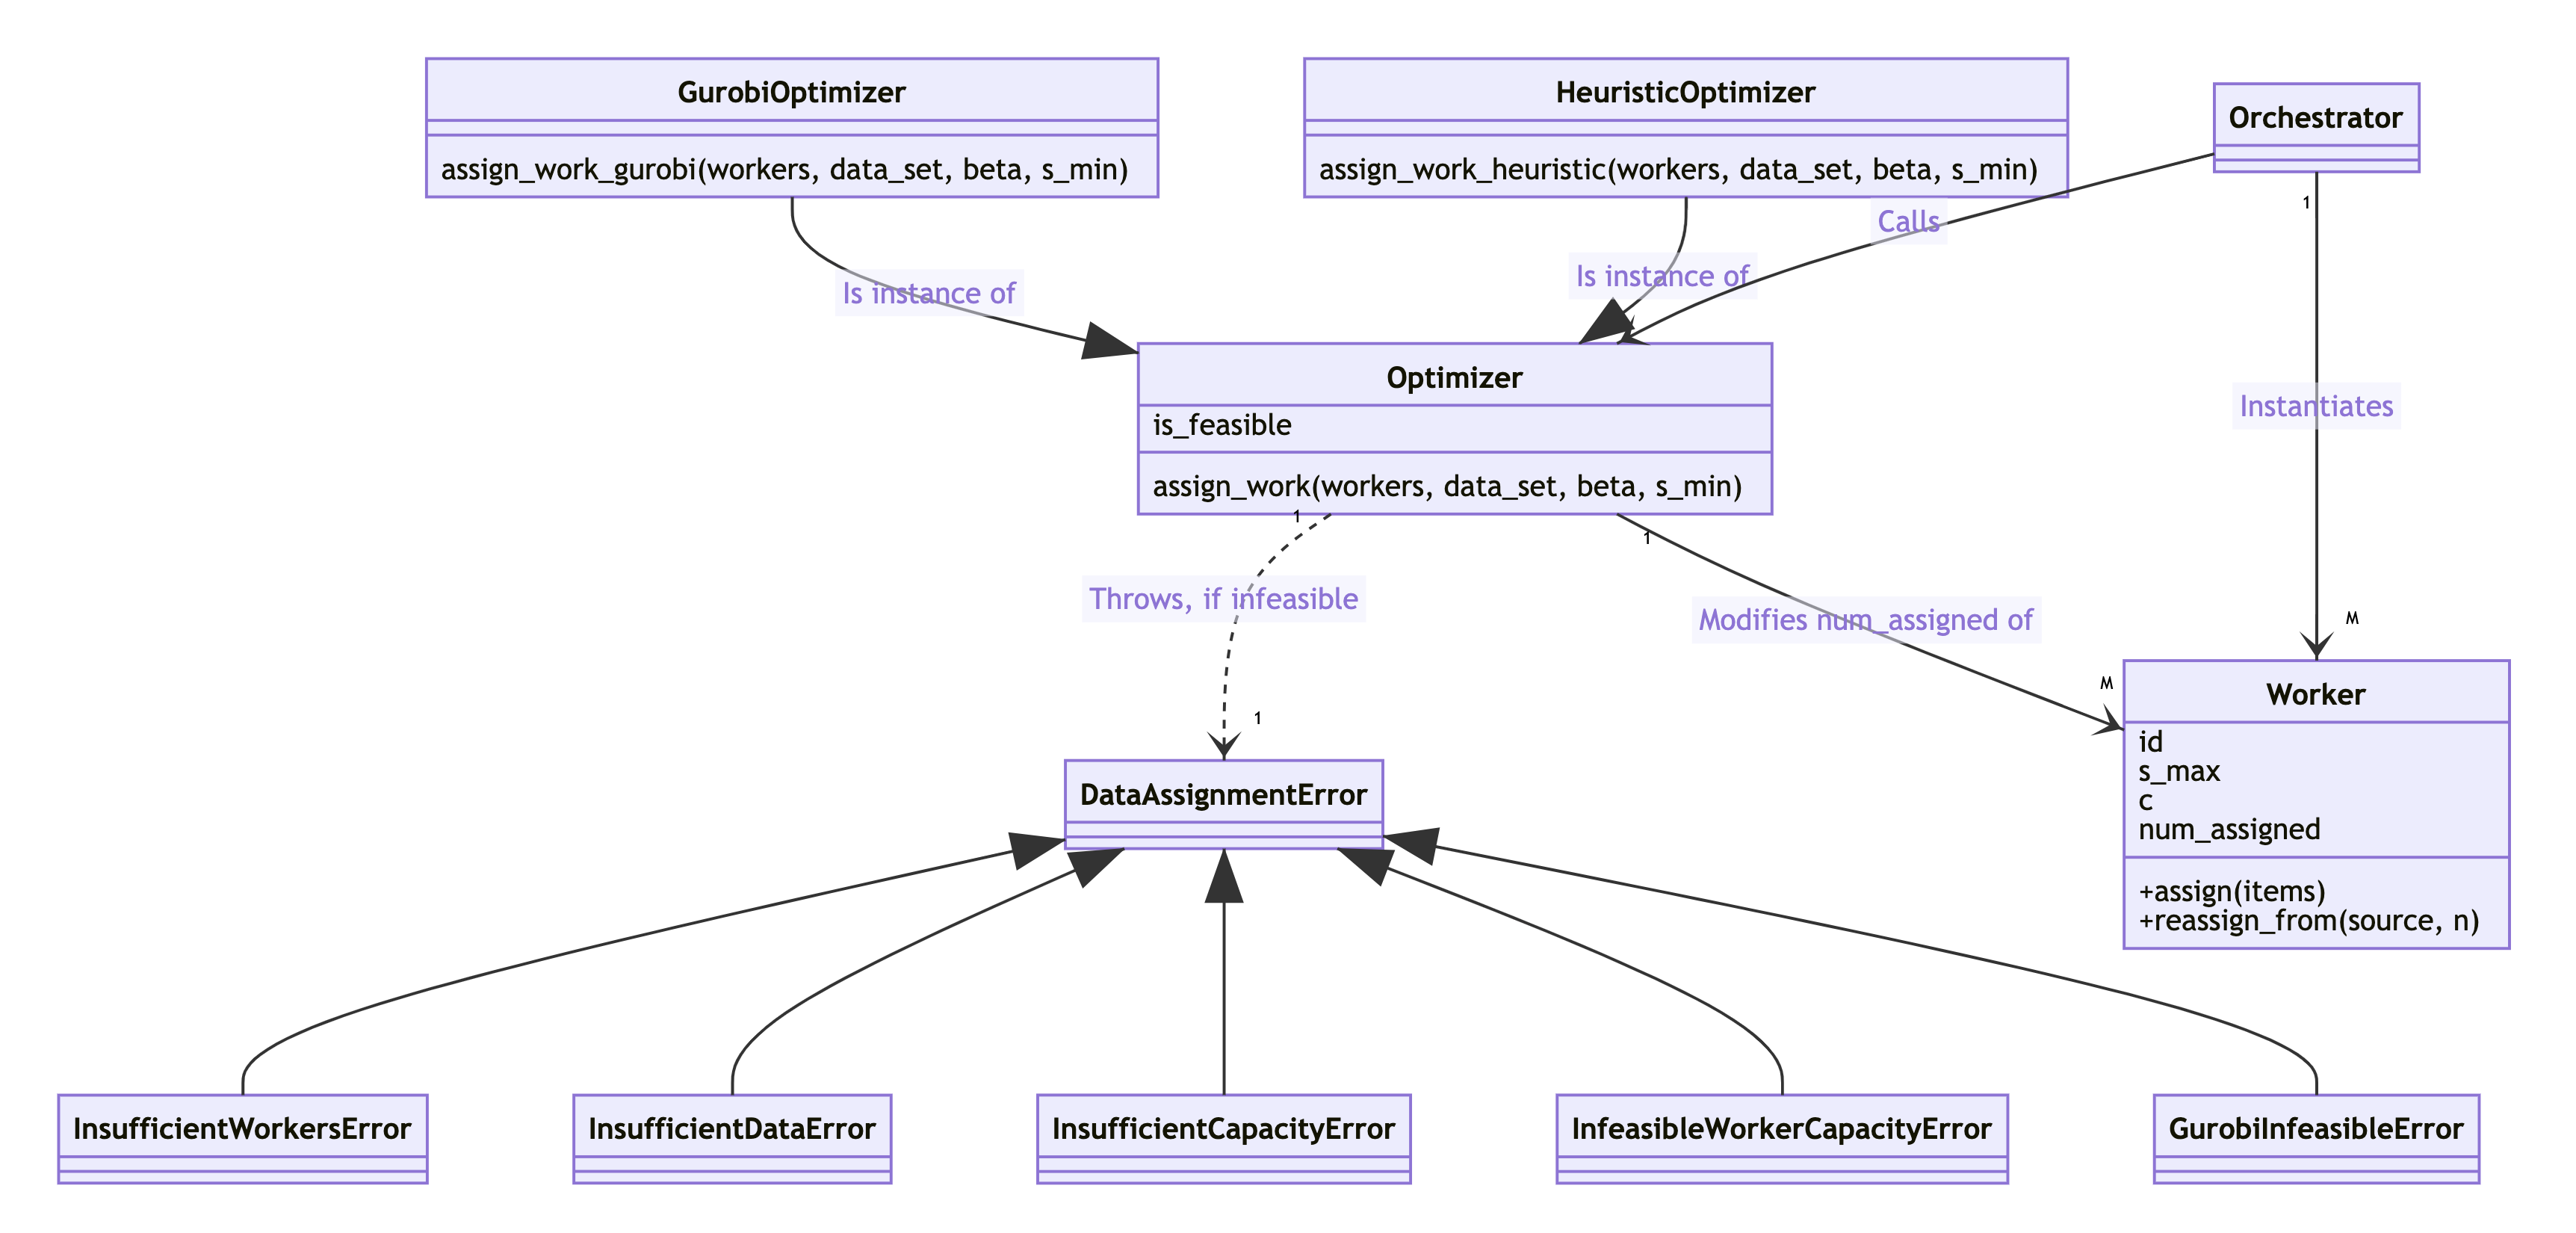
\includegraphics{thesis/img/data_assignment.png}
        \caption{Architecture Diagram of Optimization Implementation}
        \label{fig:optimization-architecture}
    \end{figure}
    
    In this model, the \texttt{GurobiOptimizer} represents the implementation of the Gurobi optimization solver, and \texttt{HeuristicOptimizer} represents the implementation of the heuristic algorithm. Both are instances of an \texttt{Optimizer}, meaning they both implement the same high-level functionality from the perspective of the orchestrator.
    
    Besides the obvious differences in how each optimizer determines the partition $\boldsymbol{D}$ of $D$, they also differ in the resolution of response that is provided in the case of an infeasible optimization problem.
    
    \subsection{\texttt{GurobiOptimizer}}
    \label{ssec:optimization-gurobi-optimizer-implementation}
    
    The \texttt{GurobiOptimizer} implements the MIP problem with Gurobi as stated in \autoref{ssec:optimization-problem-simplification}, i.e. including the simplifications on constraints from \eqref{eq:simplified-optimization-constraint-1} and \eqref{eq:simplified-optimization-constraint-3}. A simple check after running the solver checks whether the problem is feasible.
    
    If the problem is feasible, each learner is assigned the optimal subset $D_i \subseteq D$ according to the value of $x_i$ determined by the solver. If the problem is infeasible, a \texttt{GurobiInfeasibleError} (an instance of \texttt{DataAssignmentError}) is thrown.
    
    Herein lies the limitation in infeasible response alluded to above: \texttt{GurobiOptimizer} is only capable of indicating that a problem \textit{is} or \textit{is not} feasible, but cannot provide suggestions as to \textit{why} a problem is infeasible. Oftentimes a simple misconfiguration of system parameters ($\beta$ or $s_{min}$) result in infeasibility, but there is no way to detect this when using this optimizer. This is a result of Gurobi not understanding the semantics of the MIP problem; this is a clear disadvantage to this optimizer.
    
    \subsection{\texttt{HeuristicOptimizer}}
    \label{ssec:optimization-heuristic-optimizer-implementation}
    
    The \texttt{HeuristicOptimizer} implements a heuristic algorithm which is capable of solving the MIP problem as stated in \autoref{sec:optimization-problem-description}. The algorithm is consists of the following steps:
    
    \begin{enumerate}
        \item Inputs $D$, $\mathbf{L}$, $\beta$, $s^{min}$ as stated in \autoref{ssec:optimization-orchestrator-interface}.
        \item Let $n := \vert D \vert$, $k := \vert \mathbf{L} \vert$.
        \item Let $k_{max} := \lfloor \frac{n}{s^{min}} \rfloor$ be the \textit{maximum number of employable workers}.
        \item Assume WLOG: $n > 0$; $k > 0$; $s^{min} > 0$; $\beta > 0$. If assumption(s) fail, \textbf{raise} a general \texttt{ValueError}
        \item Check $n \geq \beta \cdot s^{min}$.
            \begin{enumerate}
                \item If false, \textbf{raise} \texttt{InsufficientDataError}
            \end{enumerate}
        \item Find $\mathbf{L}_e \subseteq \mathbf{L}$, the \textit{subset employable workers}:
            \begin{enumerate}
                \item Set $\mathbf{L}_e := \{ l_i \in \mathbf{L} : s^{max}_i \geq s^{min} \}$
                \item Let $k_e := \vert \mathbf{L}_e \vert$
                \item Reorder indices of $l_i \in \mathbf{L}_e$ such that $c_1 < c_2 < ... < c_{k_e}$
                \item If $k_e \leq k_{max}$, go to Step 7
                \item Let $\mathbf{L}_e^{all} = {\mathbf{L}_e \choose k_{max}}$ be the set of combinations of $\mathbf{L}_e$ of length $k_{max}$ in \textit{lexicographical order} given by the indices $i \forall l_i \in \mathbf{L}_e$, and denote by $N$ the size of $\mathbf{L}_e^{all}$.
                \item For $j := 1, ..., N$:
                    \begin{enumerate}
                        \item Set $\mathbf{L}_e := \mathbf{L}_{e^{all}_j}$
                        \item If $\sum_{l_i \in \mathbf{L}_e} s^{max}_i \geq n$, go to Step 7
                    \end{enumerate}
                \item Raise \texttt{InfeasibleWorkerCapacityError}
            \end{enumerate}
        \item Check $k_e \geq \beta$
            \begin{enumerate}
                \item If false, \textbf{raise} \texttt{InsufficientWorkersError}
            \end{enumerate}
        \item Check $\sum_{l_i \in \mathbf{L}_e} s^{max}_i \geq n$
            \begin{enumerate}
                \item If false, \textbf{raise} \texttt{InsufficientCapacityError}
            \end{enumerate}
        \item Let $n_{assigned} := 0$; $i^{last} := 0$
        \item Repeat while $n_{assigned} < n$:
            \begin{enumerate}
                \item Let $l_i := \mathbf{L}_{e,i^{last}}$ $x_i := \min\{s^{max}_i, n - n_{assigned}\}$
                \item Assign the next $x_i$ elements of $D$ to $l_i$
                \item Update $n_{assigned} := n_{assigned} + x_i$, $i^{last} := i^{last} + 1$
            \end{enumerate}
        \item Repeat up to $k_e$ times:
        \begin{enumerate}
            \item Let $k_c := \vert \{l_i \in \mathbf{L}_e : x_i \geq s^{min} \} \vert$
            \item If $k_c \geq \max\{\beta, i^{last} + 1\}$, return \textbf{Success}
            
        \end{enumerate}
        
    \end{enumerate}

    % \subsection{Data Allocation Optimization}
    % \label{ssec:data-allocation-optimization}
    % % Algorithm implementation. Includes all tested algos and which was selected and why. Visualizes algo's approach to the optimum. Describes code implementation.

    % \subsubsection{Qualifying Assumptions}
    % The system is designed so that the following assumptions are met to ensure the feasibility of a solution to the optimization problem.

    % \begin{enumerate}
    %     \item $k \geq \beta$ where $\beta$ is set as the minimum amount of workers to be distributed to.
    %     \item $n \geq s^{min} \cdot k$
    %     \item $s_i^{max} \geq s^{min}$ for $i = 1,..,k$
    %     \item $n \leq \sum_{i=1}^k s_i$, ensuring there is enough combined compute capacity to accept the entire data set.

    % \end{enumerate}

    % \subsubsection{Implementation}

    % As discussed in the midterm presentation, multiple ILP algorithms will be researched, implemented, tested, and evaluated. A preliminary list of algorithms includes

    % \begin{enumerate}
    %     \item LP relaxation of the ILP problem (e.g., simplex, dual simplex)
    %     \item Branch and cut method with LP (e.g., simplex, dual simplex)
    %     \item Hill climbing technique
    % \end{enumerate}

    % \subsubsection{Heuristic Algorithm}
    % The following is a heuristic algorithm for achieving an optimal solution to the problem.

    % \textbf{Assumptions without loss of generality}
    % \begin{enumerate}
    %     \item $s_i^{max}$, $s_{min}$, $n$, and $k$ are nonnegative integers.
    %     \item $0 \leq c_1 \leq c_2 \leq ... \leq c_k$ Otherwise rearrange the terms.
    % \end{enumerate}

    % \textbf{Procedure}
    % \begin{enumerate}
    %     \item If \[ \sum_{i=1}^k s_i = n, \] then $x_i = s_i$, $i = 1,...,k$ is the optimal solution.
    %     \item If \[\sum_{i=1}^k s_i > n,\] then let $x_i = s^{min}$ for $i = 1,...,k$.
    %     \item Set $l = 1$. Add 1 to $x_l$ until $x_l = s_l^{max}$, then let $l = l+1$ and repeat. Continue until \[ \sum_{i=1}^{k} x_i = n \]. This yields the optimal solution.
    % \end{enumerate}

    \section{Parallel Learning}
    \label{sec:parallel-learning}
\end{document}
